% !TEX root = tnnls_depression_survey.tex

\ifx\allfiles\undefined
    \input{tnnls_prefix}
\fi

\section{Introduction}
%%%%%%%%%%%%%%%%%%%%%%%%%%%%%%%%%%%%%%%%%%%%%%%%%%%%%%%
%%%%%%%%%%%%%%%%%%%%%%%%%%%%%%%��ͮ������֪ʶǨ�ƣ�%%%%%%%%%%%%%%%%%%%%%%%%%%%%%%%%%%%%%%%%%%%%%%%%%
%Depression were the most common mental disorders, which brought great challenge to personal wellbeing and social economy around the world. According to World Health Organization (WHO), people with mental illness are among the main victims of the Covid-19 pandemic, with worldwide cases of depression rising by more than 25\% during the pandemic. Depression is a mental illness that does not directly lead to death, but many depressed people are unable to overcome their psychological barriers and choose to commit suicide. According to statistical surveys, the probability of suicide in depression is around 10-15\%. Given the high prevalence of depression and the risk of suicide, it is becoming increasingly important to find new diagnostic and treatment protocols.
%%%%%%%%%%%%%%%%%%%%%%%%%%%%%%%%%%%%%%%%%%%%%%%%%%%%%%%%%%%%%%%%%%%%%%%%%%%%%%%%%


Depression is one of the most common mental disorders~\cite{world2017depression,bhugra2004globalisation,rao2008understanding}, affecting more than $300$ million people worldwide~\cite{wang2021social}.
Persistent grief, losing interest in things usually enjoyed, and the inability to participate in daily activities are characteristics of depression~\cite{peveler2002depression}.
Additionally, it will make patients feel poorly and lose their living ability\cite{singh2009loneliness}.
Worse still, patients with severe symptoms have thoughts of self-harm or suicide~\cite{eisenberg2007prevalence,bergfeld2018treatment,hemming2019alexithymia}.
It is estimated that nearly 70\% of depressed patients have had suicidal thoughts, and over 50\% have self-harmed\cite{huang2019prevalence}.
In short, the dangers of depression are staggering.

To alleviate the damage caused by depression, a timely and effective diagnosis is essential. However, there are three main challenges in the clinical diagnosis of depression:
(1) \emph{Objective indicators insufficient:}
Unlike other physiological diseases, there are no objective and precise markers to assess depression, such as biochemical test indicators, physiological data, or medical imaging.
Clinicians draw conclusions based on the clinical diagnostic criteria, their professional experience, and the patient's clinical presentation~\cite{faust1988expert}.
However, many patients purposely hide their actual illness while refusing to participate in treatment, which leads to skewed diagnostic outcomes.
(2) %Serious shortage of medical resources. At present, there is a serious shortage of medical professionals and medical resources for the diagnosis and treatment of depression. In particular, in low- and middle-income countries, up to 75\% of patients do not receive timely diagnosis and treatment. In addition, face-to-face psychiatric consultations are time-consuming and inefficient, further exacerbating the shortage of resources for psychiatric treatment~\cite{cheng2022addressing,butryn2017shortage}.
\emph{Medical resource shortage:}
There is a severe shortage of medical professionals and medical resources for
diagnosing and treating depression. Up to 75\% of patients do not obtain early diagnosis and treatment, especially in low-income and middle-income countries. 
Additionally, ineffective and time-consuming face-to-face consultations with psychiatrists add to the lack of resources for psychiatric care~\cite{cheng2022addressing,butryn2017shortage}.
(3) \emph{Social discrimination:}
Because the general public has low awareness of depression, there is an underlying resistance to or avoidance of mental illness.
Given this, early signs of depression may be dismissed or disregarded, losing the ideal window for treatment, which will make the condition worse and make therapy more challenging~\cite{finch2000perceived,lauber2005recommendations,angermeyer2011biogenetic,pescosolido2013backbone}.
%To alleviate the damage caused by depression, timely and effective diagnosis is essential.
%However, there are four main challenges in the clinical diagnosis of depression:
%(1) Lack of valid and accurate objective indicators. In contrast to other physiological disorders, there are no objective and specific biochemical indicators, physiological signal data, or medical imaging to diagnose and quantify depression. Clinicians can only diagnose depression by interviewing patients, and at the same time, some patients do not cooperate with the diagnosis and deliberately conceal their true state, resulting in biased or misdiagnosed findings.
%
%
%
%However, there are various issues that need to be addressed in the clinical diagnosis of depression.
%On the one hand, compared to other physical diseases, there are no objective and specific biochemical indicators, physiological signal data, or medical imaging for diagnosing and quantifying depression.
%The clinician can only make a diagnosis by interviewing the patient and using assessment scales~\cite{faust1988expert}, which depend on the patient's level of cooperation.
%Nonetheless, social discrimination may make depressed people feel stressed\cite{finch2000perceived,lauber2005recommendations,angermeyer2011biogenetic,pescosolido2013backbone}.
%When face-to-face communication with a doctor or filling in the questionnaire, they may deliberately conceal some facts and that will lead to misdiagnosis.
%On the other hand, there is a severe shortage of professional psychiatrists required for the traditional diagnosis of depression worldwide\cite{cheng2022addressing,butryn2017shortage}, which prevents many patients from being diagnosed and treated promptly.


\begin{figure}
\centering
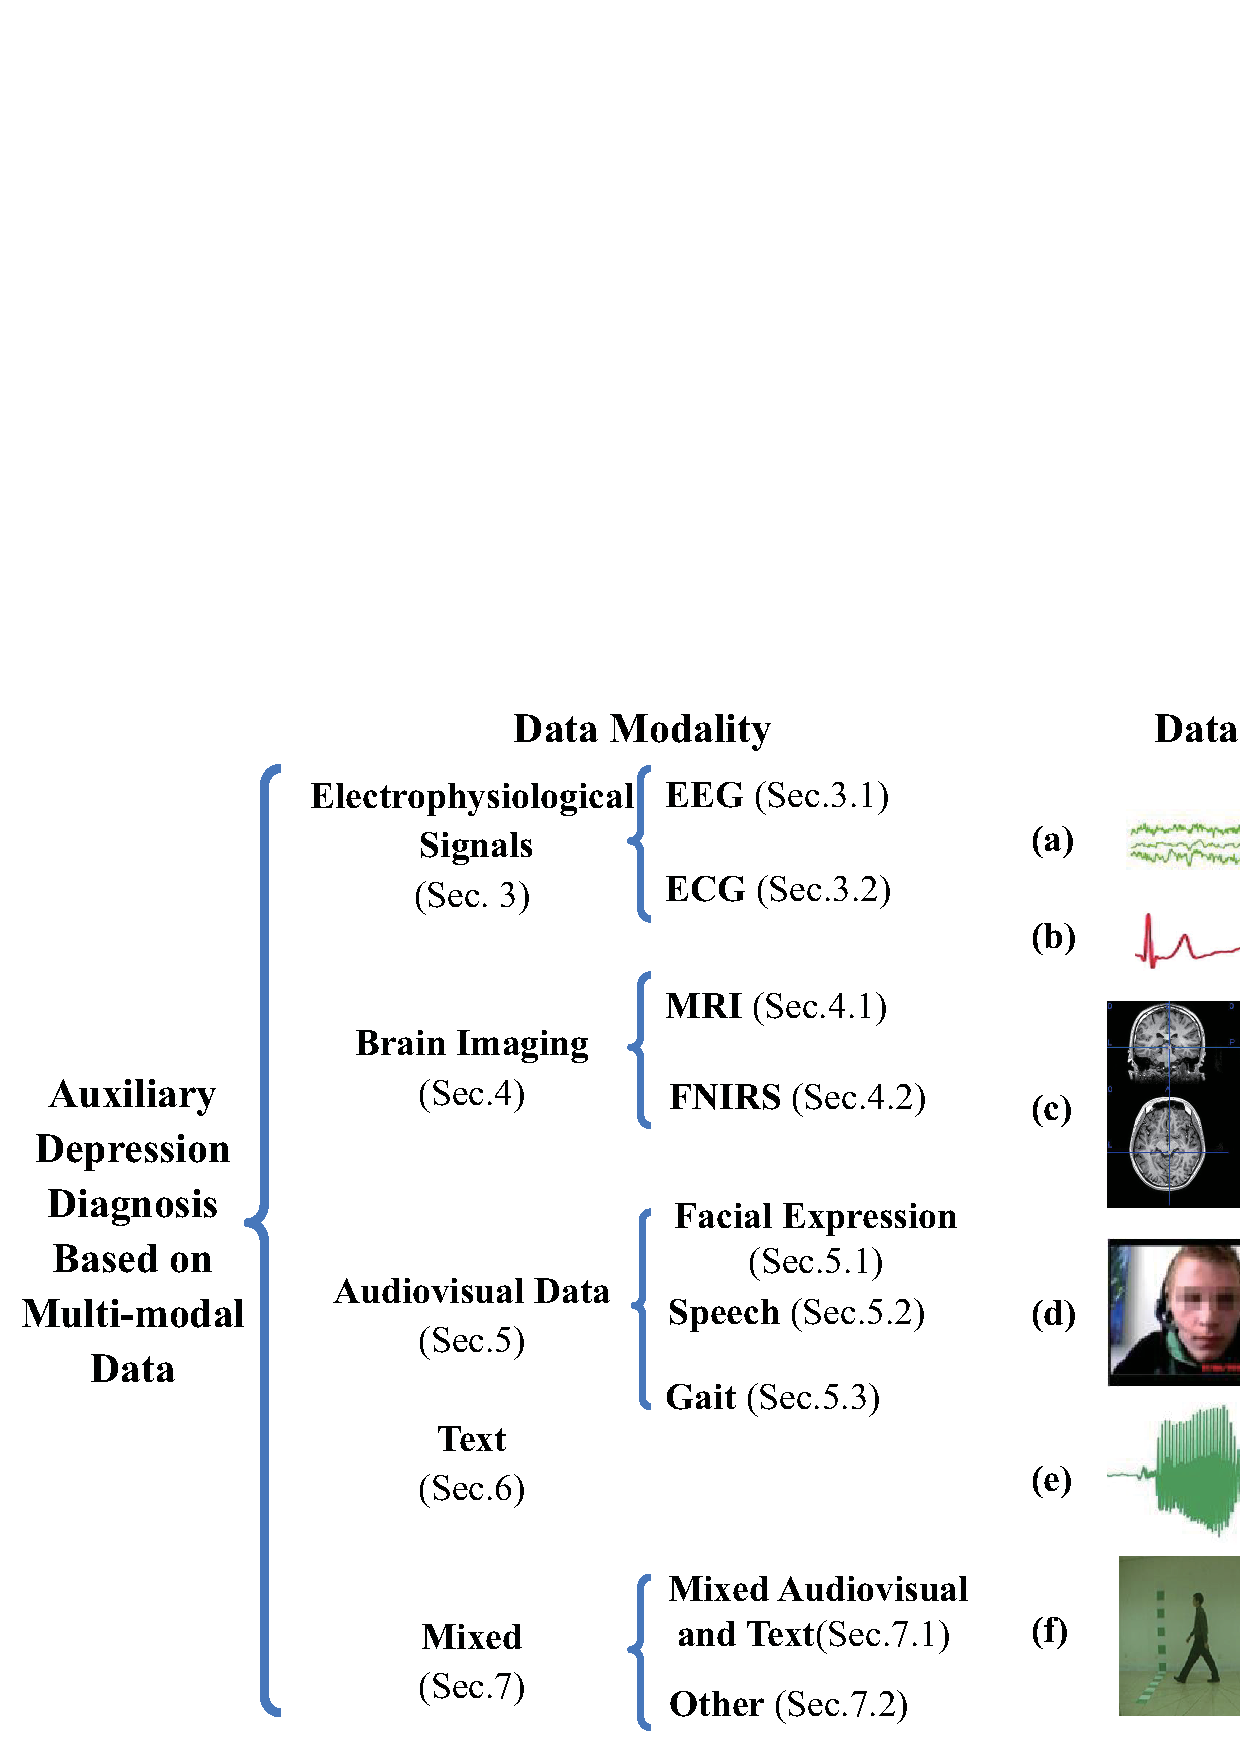
\includegraphics[width=0.9\linewidth]{figures/depression/Taxonomy.jpg}
\caption{The taxonomy of auxiliary depression diagnosis with data modality.}
%\caption{The taxonomy of auxiliary diagnosis of depression from the perspective of various categories of data.}
\label{Taxonomy}
\end{figure}
%recent ancillary diagnosis of depression (ADD) studies about the application of machine learning on various categories of data
%The taxonomy of occluded person Re-ID methods from the perspective of issues and solutions.



%The subjective factors of doctors or patients may cause misjudgements, which have an impact on the assessment of depression risk, and the search for objective methods has become the focus of research.
%In response to this circumstance, researchers have carried out studies on the evaluation of depression risk from several angles.
%By comparing the differences in physiological indicators and communication feedback exhibited between depressed and healthy people, they propose a series of machine learning-based methods to assist in depression identification.
%These methods focus on \emph{brain imaging}\cite{schnyer2017evaluating,sato2015machine,ramasubbu2016accuracy,vai2020predicting,wei2021functional},  \emph{electrophysiological signals}\cite{nilsonne2021eeg,shim2019machine,jiang2016predictability,li2016classification,kim2018automatic}, \emph{Audiovisual data}\cite{ma2016depaudionet,zhou2018visually,miao2021automatic},
%\emph{text}\cite{trotzek2018utilizing,park2015manifestation,yang2020big}, and \emph{multi-modal data}\cite{yang2017hybrid}.


%To address the difficulty of clinical diagnosis of depression, in recent years, researchers have proposed massive machine learning approaches based on the premise of comparing physiological indicators differences between depressed and healthy ones~\cite{luo2016big}.
%It not only avoids misdiagnosis or underdiagnosis due to patient non-cooperation to a large extent but also dramatically improves the efficiency of clinical diagnosis, reduces healthcare costs, and alleviates the shortage of healthcare resources.


%To address the difficulty of clinical diagnosis of depression, in recent years, researchers have proposed massive machine learning approaches. With the help of machine learning, researchers extract effective features from depression patient data automatically, and then tap the intrinsic connection between depression clinical symptoms and patients' physiological signals, which has become an important direction for auxiliary diagnosis of  depression
To address the difficulty of clinical diagnosis of depression, in recent years, researchers have proposed massive machine learning approaches.
With the help of machine learning, researchers extract practical features from depression data automatically and tap the intrinsic connection between depression clinical symptoms and physiological signals, which has become an essential direction for auxiliary depression diagnosis~\cite{luo2016big}.
The following advantages exist for machine learning-based auxiliary depression diagnosis:
(1) High efficiency: by using computer technology to analyze the physiological signals of depressed patients and create objective diagnostic indicators, clinical diagnosis can make much more quickly and effectively. 
(2) Low interference: the automatic auxiliary depression diagnosis uses a machine learning method, which eliminates the need for professionals to observe consciousness
Moreover, it lessens the difficulties of diagnosing and treating depression owing to patient resistance.

Despite the rapid evolution in this field, there still needs to be a systematic study to review and discuss existing progress.
To fill this gap, we conduct a thorough analysis of recent auxiliary depression diagnosis studies about the use of machine learning on data modality.
Next, the research methodology and machine learning procedures in auxiliary depression diagnosis
are outlined, and finally, the research directions and challenges for the future are presented.
As shown in Fig~\ref{Taxonomy}, we focus on the progress of the methods and potential research directions in five data modalities:~\emph{electrophysiological
signals}~\cite{schnyer2017evaluating,sato2015machine,ramasubbu2016accuracy,vai2020predicting,wei2021functional},  \emph{brain imaging }~\cite{nilsonne2021eeg,shim2019machine,jiang2016predictability,li2016classification,kim2018automatic}, \emph{audiovisual data}~\cite{ma2016depaudionet,zhou2018visually,miao2021automatic},
\emph{text}~\cite{trotzek2018utilizing,park2015manifestation,yang2020big}, and \emph{mixed data}~\cite{yang2017hybrid}.
%These commonly used representation forms of physiological signals are illustrated in Fig~\ref{common signals}, and we will give their brief descriptions in the following:
Fig~\ref{common signals} shows the representation forms of the corresponding physiological signals, which we will briefly describe in the following.


%%Brain function, brain structure, and brain metabolism imaging studies are the three main categories for brain imaging studies of depression.
%%%However, there are fewer structural and metabolic brain imaging investigations using depressed patients.
%%However, there are far more studies based on functional brain imaging than on the latter two.
%Brain imaging studies of depression are mainly divided into brain function, brain structure, and brain metabolism imaging studies. However, there are far more studies based on functional brain imaging of depressed patients,
%which mainly focus on dysfunction in the frontal lobe\cite{zhang2018multi,yamamura2016association,huang2017altered}, temporal lobe\cite{rolls2018effective}, amygdala\cite{zhu2018abnormal}, and cingulate gyrus\cite{gbyl2019cortical}.
%Functional magnetic resonance imaging (fMRI) is currently the main tool for studying functional brain imaging.


(1) \emph{Electrophysiological signals:}
Electrophysiological signals are caused by changes in the membrane potential of individual cells~\cite{widmann2015digital}, which are usually recorded by metal electrodes placed on the body surface.
Electroencephalography (EEG, tracing brain tissue activities), electrocardiography (ECG, recordings of the cardiac movement), and electrooculogram (EOG, examining the behavior of eyes) are common electrophysiological signals relevant to clinical interest.
They have wide application in auxiliary depression diagnosis due to their non-invasive detection and simplicity of use.

(2) \emph{Brain imaging:}
Brain imaging refers to the usually non-invasive or minimally invasive techniques that enable imaging the structure or function of the brain~\cite{lenartowicz2017brain}. It is achieved by scanning the subject's brain with various precision instruments.
Functional Near-Infrared Spectroscopy (fNIRS), nuclear Magnetic Resonance Imaging (MRI), etc., are its primary data representations.
Studies have shown that, to some extent, brain imaging can identify different types of depression depending on the affected parts of the brain~\cite{nestler2002neurobiology}.

%Electrophysiological signals, which mainly include EEG,
%ECG, EOG, galvanic skin response, and body temperature,
%have been used extensively to diagnose depression because of
%their non-invasive detection and ease of use
% These signals arise from the membrane potential changes of electrically active cells, e.g., neurons in the brain controlling bodily functions, muscle cells enabling motion, pacemaker cells governing heart rhythm, and pancreatic cells responsible for insulin release. The common electrophysiological signals that are of clinical interest are electrocardiography (ECG, recordings of the cardiac movement), electroencephalography (EEG, tracing brain tissue activities), and electromyography (EMG, examining the behavior of muscle fibers or cells).

%Apart from using fMRI to assist in diagnosing depression, electrophysiological signals, especially electroencephalography(EEG), electrocardiography(ECG), electrodermal (EOG), and body temperature, have also received extensive attention\cite{trambaiolli2020resting}.
%EEG signals are most commonly used among them because of their great temporal resolution and sensitivity to minute changes in brain activity \cite{zeng2018eeg}.
%EEG-based methods for depression identification currently mostly use feature extraction with traditional classifier geometry, and some studies have also focused on convolutional neural networks.


%Electrophysiological signals to assist in the diagnosis of depression has also been heavily researched, mainly including electroencephalography, electrocardiography, electrodermal, gastric, ophthalmic, and body temperature. Among these, EEG signals are used most frequently due to their high temporal resolution and sensitivity to slight changes in brain activity [34]. EEG-based methods for depression identification currently mostly use feature extraction with traditional classifier geometry, and some studies have also focused on convolutional neural networks.


(3) \emph{Audiovisual data:}
Audiovisual data, whose forms mainly include facial expressions, speech, and gait, are captured by video and audio recording devices. 
Depression's clinical manifestations include slower movement and speech, which can be caught audio-visually and serve as a valuable tool for an auxiliary depression diagnosis.
%{\color{red}
%Audiovisual data-based auxiliary depression diagnosis is the first recognition method proposed by researchers and the most widely used method, which has the advantage of low acquisition cost but can achieve better recognition results.
%}
%The audiovisual data based method was the first method proposed by researchers for ADD and is the most widely used method, with the advantage of low acquisition cost but better recognition results.



%Many researchers have used facial expression, speech, and gait to diagnose depression because depressed patients always exhibit abnormal behavior, such as sluggish facial expressions\cite{dai2012more}, frequent avoidance of eye contact, and speaking in short sentences with a flat tone\cite{kraepelin1921manic}. The model is more accurate based on the ease of obtaining data.

(4) \emph{Text:}
Text is the most direct medium for people to express their thoughts and emotions. Especially on social media platforms, people are more inclined to express their true feelings. Therefore, numerous academics have looked at the disparities in textual expression between depressed people and those without depression in the setting of social media platforms from a textual perspective~\cite{thomee2011mobile}.


(5) \emph{Mixed:}
%In addition to utilizing single physiological or behavioural data for auxiliary depression diagnosis, many studies have sought to employ mixed data for this task.
%Mixed data have more features than unimodal data, which can give a more complete picture of the symptomatology of depressed patients.
In addition to utilizing single physiological or behavioral data for auxiliary depression diagnosis, many studies have sought to employ mixed data for this task~\cite{lalousis2021heterogeneity,meng2021bidirectional,toenders2022predicting}.
Mixed data have more features than unimodal data, which
can give a complete picture of the symptomatology of
depressed patients.


\begin{figure}
\centering
\includegraphics[width=1\linewidth]{figures/depression/raw_signals.jpg}
\caption{Common physiological signals: subgraphs $a-c$ represent, electrophysiological signals, brain imaging, and audiovisual data, respectively.}
%These categories, in turn, have different representations: fNIRS, MRI, EEG, ECG, EOG, facial expression, speech, and gait.
\label{common signals}
\end{figure}


In this paper, we review the current state of research on machine learning in auxiliary depression diagnosis regarding the five data modalities mentioned above, focusing on the progress and potential research directions of using machine learning techniques in their contexts.
To the best of our knowledge, this is the first comprehensive survey about auxiliary depression diagnosis on different data modalities, which will provide researchers and clinical psychologists with a better understanding of the use of machine learning in this area.
%The main contributions of this study lie in three folds.


%(1) To the best of our knowledge, this is the first comprehensive survey about auxiliary depression diagnosis on different data modalities, which will provide researchers and clinical psychologists with a better understanding of the use of machine learning in this area.
%
%(2) We provide an in-depth review of advanced auxiliary depression diagnosis studies, and compare the performance of different methods in each data modality.
%
%(3) We provide a summary and analysis of the pros and cons of several auxiliary depression diagnosis methods, as well as insights into prospective research prospects in this field.


The rest of this survey will be organized as follows: Section
2 introduces some basic knowledge in auxiliary depression diagnosis tasks, including scales, datasets, and assessment metrics.
Section 3-7 provides an in-depth analysis of machine learning-based approaches to auxiliary depression diagnosis from the perspective of different data modalities. Section 8 provides
insights into promising research directions and concludes the survey.


\ifx\allfiles\undefined
% !TEX root = tnnls_relation_gait.tex

% if have a single appendix:
%\appendix[Proof of the Zonklar Equations]
% or
%\appendix  % for no appendix heading
% do not use \section anymore after \appendix, only \section*
% is possibly needed

% use appendices with more than one appendix
% then use \section to start each appendix
% you must declare a \section before using any
% \subsection or using \label (\appendices by itself
% starts a section numbered zero.)
%

%\appendices
%\section{Proof of the First Zonklar Equation}
%Appendix one text goes here.
%
%% you can choose not to have a title for an appendix
%% if you want by leaving the argument blank
%\section{}
%Appendix two text goes here.

% use section* for acknowledgment
% \section*{Acknowledgment}
% The authors would like to thank Prof. Dongbin Zhao for his support to this work.

% Can use something like this to put references on a page
% by themselves when using endfloat and the captionsoff option.
\ifCLASSOPTIONcaptionsoff
  \newpage
\fi

% trigger a \newpage just before the given reference
% number - used to balance the columns on the last page
% adjust value as needed - may need to be readjusted if
% the document is modified later
%\IEEEtriggeratref{8}
% The "triggered" command can be changed if desired:
%\IEEEtriggercmd{\enlargethispage{-5in}}

% references section

% can use a bibliography generated by BibTeX as a .bbl file
% BibTeX documentation can be easily obtained at:
% http://mirror.ctan.org/biblio/bibtex/contrib/dsoc/
% The IEEEtran BibTeX style support page is at:
% http://www.michaelshell.org/tex/ieeetran/bibtex/
\bibliographystyle{IEEEtran}
% argument is your BibTeX string definitions and bibliography database(s)
\bibliography{IEEEabrv,tnnls_relation_gait}
% \bibliography{IEEEabrv,1}
%
% <OR> manually copy in the resultant .bbl file
% set second argument of \begin to the number of references
% (used to reserve space for the reference number labels box)
%\begin{thebibliography}{1}
%\bibitem{IEEEhowto:kopka}
%H.~Kopka and P.~W. Daly, \emph{A Guide to \LaTeX}, 3rd~ed.\hskip 1em plus
%  0.5em minus 0.4em\relax Harlow, England: Addison-Wesley, 1999.
%\end{thebibliography}

% biography section
%
% If you have an EPS/PDF photo (graphicx package needed) extra braces are
% needed around the contents of the optional argument to biography to prevent
% the LaTeX parser from getting confused when it sees the complicated
% \includegraphics command within an optional argument. (You could create
% your own custom macro containing the \includegraphics command to make things
% simpler here.)
%\begin{IEEEbiography}[{\includegraphics[width=1in,height=1.25in,clip,keepaspectratio]{mshell}}]{Michael Shell}
% or if you just want to reserve a space for a photo:

%\begin{IEEEbiography}{Michael Shell}
%Biography text here.
%\end{IEEEbiography}
%
%% if you will not have a photo at all:
%\begin{IEEEbiographynophoto}{John Doe}
%Biography text here.
%\end{IEEEbiographynophoto}

% insert where needed to balance the two columns on the last page with
% biographies
% \newpage

%\begin{IEEEbiographynophoto}{Jane Doe}
%Biography text here.
%\end{IEEEbiographynophoto}


% You can push biographies down or up by placing
% a \vfill before or after them. The appropriate
% use of \vfill depends on what kind of text is
% on the last page and whether or not the columns
% are being equalized.

%\vfill

% Can be used to pull up biographies so that the bottom of the last one
% is flush with the other column.
%\enlargethispage{-5in}

% that's all folks
\end{document} 
\fi
